\documentclass[letterpaper,oneside]{book}
%\documentclass[letterpaper,twoside]{book}
% the two-column setup looks better for letter paper with a larger width.
\usepackage{geometry}
\geometry{margin=1.5cm, vmargin={0pt,1cm}}
\setlength{\topmargin}{-1cm}
\setlength{\paperheight}{29.7cm}
\setlength{\textheight}{25.1cm}

% auto adjust the marginals
\usepackage{marginfix}

%\usepackage[algo2e,lined,boxed,linesnumbered]{algorithm2e}

\usepackage{algorithm}
\usepackage{algpseudocode}
\usepackage{subcaption}
\usepackage{graphicx}

\usepackage{amsfonts}
\usepackage{amsmath}
\usepackage{amssymb}
\usepackage{amsthm}
%\usepackage{CJKutf8}
\usepackage{enumerate}
\usepackage{enumitem}
\usepackage{fancyhdr}
\usepackage{graphicx}
\usepackage{caption}
\usepackage{float}
\usepackage{layout}
\usepackage{lineno}
\usepackage{makeidx}
\usepackage{mathrsfs}
\usepackage[version=4]{mhchem}
\usepackage{lipsum}
\usepackage{multicol,caption}
\usepackage{natbib}
%\usepackage{subfigure}
\usepackage{tcolorbox} % this package is needed for \voidenvironment below
\usepackage{tikz}
\usepackage{multirow}
\usetikzlibrary{arrows,automata,backgrounds,cd}
\usetikzlibrary{shapes,snakes}

\newcommand{\Rx}[1]{\mathrm{R}[#1]}
\newcommand{\Lx}[1]{\mathrm{L}[#1]}
\newcommand{\Ux}[1]{\mathrm{U}[#1]}
\newcommand{\Dx}[1]{\mathrm{D}[#1]}
\newcommand{\Cx}[1]{\mathrm{C}[#1]}
\newcommand{\Sx}[1]{\mathrm{S}[#1]}

\newcommand{\ccg}[1]{\overline{#1}}
\newcommand{\dif}{\mathrm{d}}
\newcommand{\Dim}{\mathrm{D}}
\newcommand{\avg}[1]{\left\langle #1 \right\rangle}
\newcommand{\innerProd}[1]{\left\langle #1 \right\rangle}
\newcommand{\cond}{\mathrm{cond}}
\newcommand{\Cond}[2]{\mathrm{cond}_{#1}\left(#2\right)}
\newcommand{\difFrac}[2]{\frac{\dif #1}{\dif #2}}
\newcommand{\gen}[1]{\left\langle #1 \right\rangle}
\newcommand{\ii}{\mathbf{i}}
\newcommand{\Imz}{\mathrm{Im}\,}
\newcommand{\Int}{\mathrm{Int}}
\newcommand{\Ext}{\mathrm{Ext}}
\newcommand{\Cl}{\mathrm{Cl}}
\newcommand{\Fr}{\mathrm{Fr}}
\newcommand{\Ker}{\mathrm{ker}}
\newcommand{\pdfFrac}[2]{\frac{\partial #1}{\partial #2}}
\newcommand{\Rez}{\mathrm{Re}\,}
\newcommand{\sgn}{\mathrm{sgn}}
\newcommand{\Span}{\mathrm{span}}
\newcommand{\OFL}{\mathrm{OFL}}
\newcommand{\UFL}{\mathrm{UFL}}
\newcommand{\fl}{\mathrm{fl}}
%\newcommand{\op}{\mathrm{op}}
\newcommand{\op}{\odot}
\newcommand{\Eabs}{E_{\mathrm{abs}}}
\newcommand{\Erel}{E_{\mathrm{rel}}}
\newcommand{\dom}{\mathrm{dom}}
\newcommand{\Null}{\mathrm{null}}
\newcommand{\Range}{\mathrm{range}}
\newcommand{\Supp}{\mathrm{supp}}
\newcommand{\Arity}{\mathrm{arity}}
\newcommand{\by}[1]{\boldsymbol{#1}}

\newenvironment{Figure}
{\par\medskip\noindent\minipage{\linewidth}}
{\endminipage\par\medskip}

% this environment is for solutions of examples and exercises
\newenvironment{solution}%
{\noindent\textbf{Solution.}}%
{\qedhere}
% the following command is for disabling environments
%  so that their contents do not show up in the pdf.
\makeatletter
\newcommand{\voidenvironment}[1]{%
  \expandafter\providecommand\csname env@#1@save@env\endcsname{}%
  \expandafter\providecommand\csname env@#1@process\endcsname{}%
  \@ifundefined{#1}{}{\RenewEnviron{#1}{}}%
}
\makeatother



%----------------------------------------
% theorem and theorem-like environments %
%----------------------------------------
\numberwithin{equation}{chapter}
\theoremstyle{definition}

\newtheorem{thm}{Theorem}[chapter]
\newtheorem{alg}[thm]{Algorithm}
\newtheorem{asm}[thm]{Assumption}
\newtheorem{axm}[thm]{Axiom}
\newtheorem{coro}[thm]{Corollary}
\newtheorem{defn}[thm]{Definition}
%\newtheorem{exm}{Example}[chapter]
%\newtheorem{exc}[exm]{Exercise}
% number examples and exercises with thms.
\newtheorem{exm}[thm]{Example}
\newtheorem{exc}[thm]{Exercise}
\newtheorem{frm}[thm]{Formula}
\newtheorem{lem}[thm]{Lemma}
\newtheorem{ntn}{Notation}
\newtheorem{prop}[thm]{Proposition}
\newtheorem{rem}{Remark}[chapter]
\newtheorem{rul}[thm]{Rule}



%%%%%%%%%%%%%% for INSE %%%%%%%%%%%%%
\usepackage{bm}
\usepackage[sans]{dsfont}
\usepackage{url}
\newcommand{\ibold}{{\mathbf{i}}}
\newcommand{\jbold}{{\mathbf{j}}}
\newcommand{\kbold}{{\mathbf{k}}}
\newcommand{\ebold}{{\mathbf{e}}}
\newcommand{\ubold}{{\mathbf{u}}}
\newcommand{\xbold}{{\mathbf{x}}}
\newcommand{\pbold}{{\mathbf{p}}}
\newcommand{\etabold}{\bm{\eta}}
\newcommand{\unitV}{\mathds{1}}
\newcommand{\zerobold}{{\mathbf{0}}}
\newcommand{\dt}{{\Delta t}}
\newcommand{\avgI}[1]{\langle #1 \rangle_{\ibold}}
\newcommand{\iphed}{{\ibold+\frac{1}{2}\ebold^d}}
\newcommand{\imhed}{{\ibold-\frac{1}{2}\ebold^d}} %new
% i plus fractional e^d
\newcommand{\ipfed}[1]{\ibold+\frac{#1}{2}\ebold^d}
% i minus fractional e^d
\newcommand{\imfed}[1]{\ibold-\frac{#1}{2}\ebold^d}
\newcommand{\ipmfed}[1]{\ibold\pm\frac{#1}{2}\ebold^d}
\newcommand{\half}{\frac{1}{2}}
\newcommand{\Lapl}{{\mathbf{L}}}
\newcommand{\Div}{{\mathbf{D}}}
\newcommand{\Grad}{{\mathbf{G}}}
\newcommand{\Iden}{{\mathbf{I}}}
\newcommand{\nref}{n_{\text{ref}}}
\newcommand{\phio}{\phi^{\circ}}
\newcommand{\eq}[1]{(\ref{#1})}
\newcommand{\Proj}{{\mathbf{P}}}
\newcommand{\cProj}{{\mathcal{P}}}
\newcommand{\cProjLH}{{\mathscr{P}}}
\newcommand{\ProjAux}{{\mathbf{Q}}}
\newcommand{\exOp}{{\mathbf{X}}^{[\text{E}]}}
\newcommand{\imOp}{{\mathbf{X}}^{[\text{I}]}}
\newcommand{\nStages}{n_{\tiny \textsf{s}}}
\newcommand{\mb}[1]{\mathbf{#1}}
%%%%%%%%%%%%%%%%%%%%%%%%%%%%%%%%%
\newcommand{\fYear}{2025}

\usepackage{ctex}
\usepackage{booktabs}   % 表格排版
%\makeindex
  
\begin{document}
\pagenumbering{roman}

%\thispagestyle{empty}
\begin{small}
\tableofcontents
\end{small}

% --------------------------------------------------------
% uncomment the following to remove these environments 
%  to generate handouts for students.
% --------------------------------------------------------
\begingroup
%\voidenvironment{rem}%
%\voidenvironment{proof}%
%\voidenvironment{solution}%
% \input{sec/methodsOfStudy}

%\setcounter{chapter}{-1}
\pagenumbering{arabic}

\setcounter{page}{1}

%\clearpage

% This page has been intentionally left blank.

% \clearpage

\pagestyle{fancy}
\fancyhead{}
\lhead{木子}
\chead{Reinforcement Learning}
\rhead{\fYear}
\chapter{LLMs 的强化学习基础}
%\begin{multicols}{2}
%\setlength{\columnseprule}{0.2pt}
% \begin{rem}
%   Based on the universal approximation theorem, the MLPs play a
%   significant role in the field of deep learning.
%\end{rem}
\section{RL 基础介绍}
强化学习的核心是智能体(Agent)与环境(Environment)的交互学习框架,其基本要素包括:
\begin{enumerate}%[leftmargin=2.5cm]
  \item \textbf{状态(State)} 环境在时刻$t$的观测表示,记为$S_t \in \mathcal{S}$。例如:\\
  - 机器人坐标 $(x,y)$ \\
  - 棋盘局面的矩阵编码
  
  \item \textbf{动作(Action)} 智能体在状态$s$下的可执行操作,记为$A_t \in \mathcal{A}(s)$。例如:\\
  - 离散动作:围棋的落子位置 \{上, 下, 左, 右\} \\
  - 连续动作:机械臂关节扭矩 $[0, 1]^n$
  
  \item \textbf{奖励(Reward)} 环境对动作的即时反馈,记为$R_{t+1} \in \mathbb{R}$。例如:\\
  - 游戏得分变化:$+1$(得分),$-10$(触碰障碍) \\
  - 稀疏奖励:仅在任务完成时获得$+100$
\end{enumerate}

% ================================================
\subsection{马尔可夫决策过程(MDP)}
\textbf{马尔可夫性}:未来状态仅依赖当前状态与动作:
\[
P(S_{t+1}|S_t, A_t) = P(S_{t+1}|S_t, A_t, S_{t-1}, A_{t-1}, \dots).
\]
MDP五元组定义为:
\[
\langle \mathcal{S}, \mathcal{A}, P, R, \gamma \rangle:
\]
\begin{itemize}%[leftmargin=2.5cm]
  \item $\mathcal{S}$ 状态空间(有限或无限集合)
  \item $\mathcal{A}$ 动作空间(可能依赖状态$s$)
  \item $P(s'|s,a)$ 状态转移概率:$\sum_{s'} P(s'|s,a) = 1$
  \item $R(s,a,s')$ 奖励函数(可简化为$R(s,a)$或$R(s)$)
  \item $\gamma$ 折扣因子:$\gamma=0$只关注即时奖励,$\gamma \to 1$强调长期回报
\end{itemize}

强化学习的目标即是在此框架下最大化\textbf{累积折扣奖励}:
\begin{equation}
  G_t = \sum_{k=0}^{\infty} \gamma^k R_{t+k+1}
\end{equation}
优化策略$\pi(a|s)$以最大化期望回报$\mathbb{E}_\pi[G_t]$。

% ================================================
\subsection{价值函数与贝尔曼方程}
\subsubsection{状态价值函数(State-Value Function)}
策略$\pi$下状态$s$的长期价值,定义为从$s$出发的期望回报:
\[
V^\pi(s) = \mathbb{E}_\pi \left[ G_t \mid S_t = s \right]
\]
其中累积回报:
\[
G_t = \sum_{k=0}^\infty \gamma^k R_{t+k+1}
\]

\subsubsection{动作价值函数(Action-Value Function)}
在状态$s$采取动作$a$后遵循策略$\pi$的期望回报:
\[
Q^\pi(s,a) = \mathbb{E}_\pi \left[ G_t \mid S_t = s, A_t = a \right]
\]

\subsubsection{贝尔曼方程(Bellman Equation)}
价值函数的递归分解:
\[
V^\pi(s) = \sum_{a} \pi(a|s) \sum_{s'} P(s'|s,a) \left[ R(s,a,s') + \gamma V^\pi(s') \right]
\]
\[
Q^\pi(s,a) = \sum_{s'} P(s'|s,a) \left[ R(s,a,s') + \gamma \sum_{a'} \pi(a'|s') Q^\pi(s',a') \right]
\]

\subsubsection{最优价值函数}
存在最优策略$\pi^*$使得:
\[
V^*(s) = \max_\pi V^\pi(s), \quad Q^*(s,a) = \max_\pi Q^\pi(s,a)
\]
满足贝尔曼最优方程:
\[
V^*(s) = \max_{a} \sum_{s'} P(s'|s,a) \left[ R(s,a,s') + \gamma V^*(s') \right]
\]
\[
Q^*(s,a) = \sum_{s'} P(s'|s,a) \left[ R(s,a,s') + \gamma \max_{a'} Q^*(s',a') \right]
\]

% ================================================
\subsection{强化学习方法分类}
\begin{table}[htbp]
  \centering
  \caption{强化学习方法对比}
  \begin{tabular}{lcc}
    \toprule
    \textbf{方法类型} & \textbf{策略表示} & \textbf{更新目标} \\
    \midrule
    基于值函数(Critic) & 隐式(如$\epsilon$-greedy) & 逼近$Q^*(s,a)$ \\
    基于策略(Actor) & 显式$\pi_\theta(a|s)$ & 最大化$J(\theta) = \mathbb{E}[G_t]$ \\
    Actor-Critic & 显式策略 + 值函数 & 策略梯度+值函数引导 \\
    \bottomrule
  \end{tabular}
\end{table}

\subsubsection{基于值函数的方法}
通过优化值函数间接改进策略,例如:
\begin{itemize}
  \item 动态规划(DP):迭代计算$V^\pi(s)$
  \item 蒙特卡洛(MC):采样轨迹估计$Q^\pi(s,a)$
  \item 时序差分(TD):结合DP与MC,如Q-learning:
  \[
  Q(s,a) \leftarrow Q(s,a) + \alpha \left[ R + \gamma \max_{a'} Q(s',a') - Q(s,a) \right]
  \]
\end{itemize}

\subsubsection{基于策略的方法}
直接参数化策略并通过梯度上升优化:
\[
J(\theta) = \mathbb{E}_{\tau \sim \pi_\theta} \left[ \sum_{t=0}^\infty \gamma^t R_t \right]
\]
梯度计算公式:
\[
\nabla_\theta J(\theta) = \mathbb{E} \left[ \sum_{t=0}^T \nabla_\theta \log \pi_\theta(a_t|s_t) G_t \right]
\]

\subsubsection{Actor-Critic框架}
\begin{itemize}
  \item \textbf{Actor}:策略$\pi_\theta(a|s)$,通过策略梯度更新
  \item \textbf{Critic}:值函数$V_w(s)$或$Q_w(s,a)$,通过TD误差更新
  \item 优势函数(Advantage Function)减少方差:
  \[
  A(s,a) = Q(s,a) - V(s) \implies \nabla_\theta J(\theta) = \mathbb{E} \left[ \nabla_\theta \log \pi_\theta(a|s) A(s,a) \right]
  \]
\end{itemize}
\section{基于 Actor 的直接策略梯度方法}
对于采样的轨迹 episode $\tau^{n}$,policy gradient 方法即是采用梯度上升方法最大化期望回报:
\begin{equation}
    \text{maximize }\mathbb{E}_{\tau\sim p(\tau|\theta)}[R(\tau)] = \sum_{\tau} R(\tau)p(\tau|\theta)
    %=\text{maximize }\frac{1}{N}\sum_{n=1}^{N}R(\tau^{n})
    =\overline{R}_\theta.
\end{equation}
其中 $\theta$ 是待优化的参数,直接计算 $\overline{R}_\theta$ 的梯度:
\begin{align}
    \nabla_\theta\overline{R}_\theta = \sum_{\tau}R(\tau)p(\tau|\theta)\frac{\nabla p(\tau|\theta)}{p(\tau|\theta)}
    = \frac{1}{N}\sum_{n=1}^{N} R(\tau^{n})\nabla\log (p(\tau^{n}|\theta)), 
\end{align}
由于
\begin{align}
    p(\tau|\theta) &= p(s_1)p(a_1|s_1,\theta)p(r_2,s_2|s_1,a_1)p(a_2|s_2,\theta)p(r_3,s_3|s_2,a_2) \cdots p(r_T,s_T|s_{T-1},a_{T-1})\\
    &=p(s_1)\prod_{t=1}^{T-1}p(a_t|s_t,\theta)p(r_{t+1},s_{t+1}|s_t,a_t),
\end{align}
因此
\begin{align}
    \nabla \log (p(\tau|\theta)) &= \sum_{t=1}^{T-1} \nabla \log(p(a_t|s_t,\theta)),\\
    \nabla \overline{R}_\theta &= \frac{1}{N}\sum_{n=1}^{N}\sum_{t=1}^{T-1}R(\tau^{n}) \nabla \log(p(a_t^n|s_t^n,\theta)).
\end{align}

这里梯度上升的直接理解就是若 $R(\tau^n)$ 为正,则增加 $p(a_t^n|s_t^n,\theta)$ 的概率,相反若为负则减小;另一方面,
即使 $R(\tau^n)$ 为正,但其中并不是每个行为策略都能导致 $R(\tau^n)$ 增加,因此有一些改进方法,如
对每个行为策略,计算该动作起到结束的奖励和作为 return,即
\begin{equation}\label{eq:actor gradient}
    \nabla \overline{R}_\theta = \frac{1}{N}\sum_{n=1}^{N}\sum_{t=1}^{T-1}(\sum_{t'=t}^{T}\gamma^{t'-t}r_{t'}^n-b) \nabla \log(p(a_t^n|s_t^n,\theta)).
\end{equation}
其中 $b$ 代表baseline,起到调整正负(策略相对好坏之分)、减小方差的作用,之后会引入优势函数(advantage function)。



\section{基于 critic 的 Q-learning 算法}
Q-learning 是一种无模型(model-free)的强化学习算法
属于基于值函数的方法。它通过学习一个 Q 值表来评估在特定状态下采取某个动作的长期期望回报,从而找到最优策略。
Q-learning 的学习目标是一个最优的动作价值函数 $Q*(s, a)$,表示在状态 $s$ 下执行动作 $a$ 后,遵循最优策略所能获得的最大累积奖励,
满足贝尔曼最优公式:
\begin{equation}
    Q*(s, a) = \mathbb{E} [r + \gamma \max_{a'} Q(s', a')|s,a],
\end{equation}
其中 $r$ 是即时奖励,$\gamma$ 是折扣因子,$s'$ 是下一个状态。

在状态和动作有限的情况下,Q-learning 可以通过迭代更新 Q 值表来找到最优策略,利用时序差分(TD)方法更新 Q 值:
\begin{equation}
    Q(s, a) \leftarrow (1-\alpha) Q(s, a) + \alpha (r + \gamma \max_{a'} Q(s', a')-Q(s, a))
\end{equation}
其中 $\alpha$ 是学习率,控制更新的步长。但存在维度灾难以及不具备泛化能力,DQN 利用神经网络拟合 Q 值函数很好的
解决了上述问题。

\subsection{DQN}
DQN 关键包括:
\begin{enumerate}
    \item \textbf{Q 函数} 状态 $s$ 和动作 $a$ 下的长期回报期望,用神经网络拟合得到。
    \item \textbf{目标网络 Target Network} 用于估计目标 Q 值,与 Q 函数共享参数(定期更新),用于减少样本方差,
    目标 Q 值为:
    \begin{equation}
        y = r + \gamma \max_{a'} Q_{\text{target}}(s', a').
    \end{equation}
    \item \textbf{经验回放 Experience Replay} 用于训练时从经验池中随机采样一批数据(优先回放重要性高的经验),提高样本利用率,减小过拟合。
\end{enumerate}

DQN 算法流程:
\begin{enumerate}
    \item 初始化 Q 函数和目标网络参数相同;
    \item 与环境交互,存储经验 $(s,a,r,s')$ 到回放缓冲区;
    \item 从回放缓冲区中随机采样一批数据 $(s,a,r,s')$,计算目标值 $y$;
    \item 使用 Q 函数拟合 $(s,a,y)$,更新 Q 函数参数;
    \item 定期更新目标网络参数。
\end{enumerate}

训练得到 Q 值后,更新策略为
\begin{equation}
    \pi(s) = \arg\max_{a} Q(s, a).
\end{equation}
当 $a$ 是连续时,可通过采样、对 $a$ 求导、修改网络架构等方式获得更新后的策略。
另外,为增加探索能力,可采用 $\epsilon-greedy$ 策略,以一定概率 $\epsilon$ 随机选择动作,其余概率选择最优动作。

DQN 的一些训练改进:
\begin{enumerate}
    \item \textbf{Double DQN} 解耦动作选择和目标 Q 值计算,缓解过度估计问题,即目标 Q 值计算如下:
    \begin{equation}
        y = r + \gamma Q_{\text{target}}(s', \arg\max_{a'} Q_{\pi}(s', a')).
    \end{equation}
    \item \textbf{Prioritized Experience Replay} 引入样本重要性,根据样本 TD 误差更新样本权重,提高样本利用率。
    \item \textbf{Dueling Network} 利用两个网络分离状态值和动作优势值,提高学习效率。
    \item \textbf{Noisy Network} 加入噪声,提高探索能力,具体为每次在和环境交互获取数据时,对每个参数添加随机噪声(如高斯噪声)以
    提高探索性,比 $\epsilon-greedy$ 更有效。
    \item \textbf{结合 MC 和 TD} 结合 Monte Carlo 和 TD 方法,利用 multi-step 策略,减小方差。
\end{enumerate}




\section{Actor-Critic 混合方法}
Actor-Critic 是结合了策略梯度(Policy Gradient) 和 值函数(Value Function) 的混合架构:
\begin{enumerate}
    \item Actor(策略网络):负责生成动作,直接优化策略函数 $\pi_{\theta}(a|s;\theta)$,使得策略函数的期望回报最大化;
    \item Critic(价值网络):评估状态或动作的价值,通过 $V(s;\phi)$ 或 $Q(s,a;\phi)$ 计算。
\end{enumerate}

在直接策略梯度算法中,方程~\ref{eq:actor gradient} 中
\begin{equation}
    G_t^n - b = \sum_{t'=t}^{T}\gamma^{t'-t}r_{t'}^n-b,
\end{equation}
其具有不稳定性,方差大,因此可利用价值网络估计的期望值进行修正,有
\begin{equation}
    \mathbb{E}(G_t^n) = Q^{\pi_{\theta}}(s_t^n,a_t^n),\quad \text{baseline} = V^{\pi_{\theta}}(s_t^n);
\end{equation}
另外,
\begin{align}
    &Q^{\pi_{\theta}}(s_t^n,a_t^n) - V^{\pi_{\theta}}(s_t^n) \\
    &=\mathbb{E}(r_t^n + \gamma V^{\pi_{\theta}}(s_{t+1}^n) - V^{\pi_{\theta}}(s_t^n))\\
    &= r_t^n + \gamma V^{\pi_{\theta}}(s_{t+1}^n) - V^{\pi_{\theta}}(s_t^n).
\end{align}
以上即是 advantage function,即在策略梯度算法中,用价值网络估计的期望回报与当前状态的价值对
蒙特卡洛方法的估计值进行修正,从而减少方差。

训练过程中,可通过正则化项使得策略网络的输出分布熵更大以增加探索性。
另外,对于动作连续的情景,可以采用 Pathwise derivative policy gradient 方法使用确定性策略优化,
具体的网络结果中,actor 网络的输入为状态,输出为动作,critic 网络的输入为 actor 网络的输出,
训练 actor 网络即是使得 critic 网络值最大化,类似于 GAN 的思想,具体训练流程如下:
\begin{enumerate}
    \item 初始化主网络 actor $\pi_{\theta}$ 和 critic $Q_{\phi}$ 和目标网络 actor $\pi_{\theta^-}$ 和 critic $Q_{\phi^-}$;
    \item 使用当前策略进行环境交互采样数据(可添加噪声增加探索性),存储到回放缓冲区;
    \item 最小化 TD 误差更新 critic 网络:
        \begin{equation}
            L(\phi) = \mathbb{E}\left[(r+\gamma Q_{\phi^-}(s',\pi_{\theta^-}(s')) - Q_{\phi}(s,a))^2\right].
        \end{equation}
    \item 沿 $Q_{\phi}$ 梯度方向更新 actor 网络:
        \begin{equation}
            L(\theta) = \mathbb{E}(Q_{\phi}(s,\pi_{\theta}(s))).
        \end{equation}
    \item 训练几步后更新目标网络。
\end{enumerate}
\section{PPO: Proximal Policy Optimization}
Actor-Critic 方法具有 on-policy 性质,需要频繁的交互采样数据,PPO 则通过重要性采样
获得 off-policy 性质从而避免大量的数据采样,同时 PPO 通过裁剪限制策略梯度更新的幅度从而
提高训练的稳定性。

\textbf{重要性采样:}当一个分布的采样困难时,使用另一个分布的采样数据代而计算均值,即
\begin{equation}
    \mathbb{E}_{x\sim p}[f(x)] = \mathbb{E}_{x \sim q}[f(x)\frac{p(x)}{q(x)}],
\end{equation}
但虽均值相同,方差却不同,只有两分布比较接近时,方差才差不多。

在 PPO 中,策略梯度为:
\begin{align}
    \nabla \overline{R}_{\theta} &= \mathbb{E}_{\tau\sim \pi_{\theta}}[R(\tau)\nabla\log\pi_{\theta}(\tau)]\\
    &= \mathbb{E}_{(s_t,a_t)\sim\pi_{\theta}}[A^{\theta}(s_t,a_t)\nabla\log\pi_{\theta}(a_t|s_t)]\\
    &= \mathbb{E}_{(s_t,a_t)\sim\pi_{\theta'}}[\frac{\pi_{\theta}(a_t,s_t)}{\pi_{\theta'}(a_t,s_t)}
    A^{\theta'}(s_t,a_t)\nabla\log\pi_{\theta}(a_t|s_t)]\\
    &= \mathbb{E}_{(s_t,a_t)\sim \pi_{\theta'}}[\frac{\pi_{\theta}(a_t|s_t)}{\pi_{\theta'}(a_t|s_t)}
    A^{\theta'}(s_t,a_t)]\\
    &= J^{\theta'}(\theta),
\end{align}
同时,PPO 的两种优化目标函数分别为:
\begin{align}
    J^{\theta'}_{PPO}(\theta) &= J^{\theta'}(\theta) - \beta KL(\theta' , \theta),\\
    J^{\theta'}_{CLIP PPO}(\theta) &= \mathbb{E}_t[\min(\frac{\pi_{\theta}(a_t|s_t)}{\pi_{\theta'}(a_t|s_t)}A^{\theta'}(s_t,a_t),
    clip(\frac{\pi_{\theta}(a_t|s_t)}{\pi_{\theta'}(a_t|s_t)},1-\epsilon,1+\epsilon)A^{\theta'}(s_t,a_t))].
\end{align}
以上,$\theta'=\theta_{old}$,另外在实际中,还有 critic 网络的训练目标以及熵正则化项等。
在大模型中,通常采用广义优势估计 (GAE),并在每个 token 的奖励中添加一个来自参考模型的 KL 惩罚:
\begin{equation}
    A_t = r(q,o_{\le t}) - \beta \log \frac{\pi_{\theta}(o_t|q,o_{< t})}{\pi_{\theta_{ref}}(o_t|q,o_{< t})} + GAE,
\end{equation}
其中 $r$ 是奖励模型。

\section{GRPO: Group Relative Policy Optimization}
GRPO 与 PPO 类似,但其放弃使用与策略模型大小相当的 critic model,而通过一组评分计算相对优势,
具体为:
\begin{align}
    J_{GRPO}(\theta) &= \mathbb{E}_{q\sim P(Q),\{o_i\}_{i=1}^G\sim \pi_{\theta_{old}}(O|q)}\\
            &\frac{1}{G}\sum_{i=1}^{G}\left(\min(\frac{\pi_{\theta}(o_i|q)}{\pi_{\theta_{old}}(o_i|q)}A_i),
            clip(\frac{\pi_{\theta}(o_i|q)}{\pi_{\theta_{old}}(o_i|q)},1-\epsilon,1+\epsilon)A_i
            -\beta \mathbb{D}_{KL}(\pi_{\theta}||\pi_{\theta_{ref}})\right),\\
            & \quad \mathbb{D}_{KL}(\pi_{\theta}||\pi_{\theta_{ref}}) = \frac{\pi_{ref}(o_i|q)}{\pi_{\theta}(o_i|q)}
            - \log\frac{\pi_{ref}(o_i|q)}{\pi_{\theta}(o_i|q)} -1,
\end{align}
其中每个 $o_i$ 有基于规则的评分 $r_i$,并且优势值的计算为:
\begin{equation}
    A_i = \frac{r_i - mean({r_1,\cdots,r_G})}{std({r_1,\cdots,r_G})}.
\end{equation}

\begin{figure}[H]
    \centering
    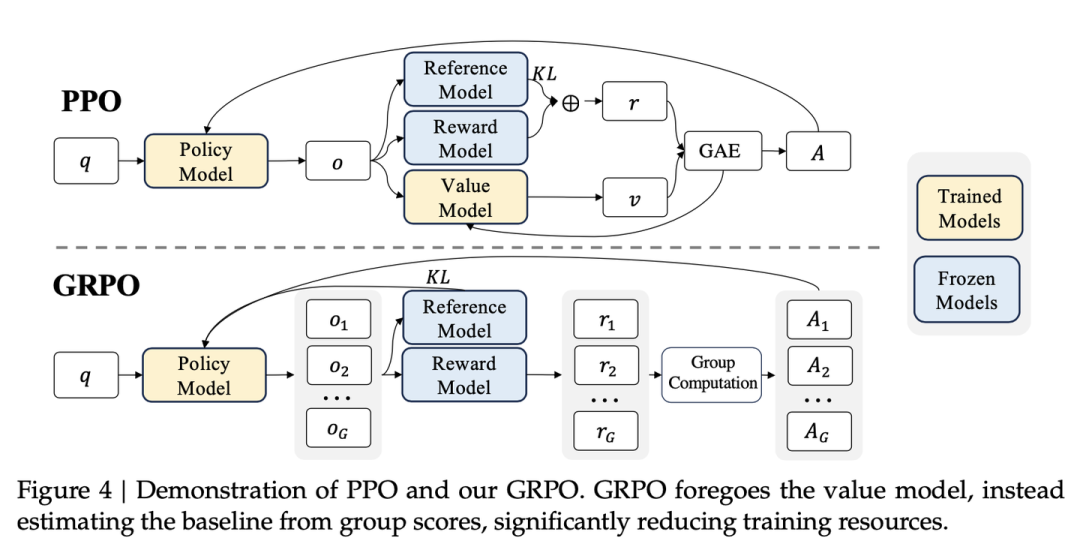
\includegraphics[width=\textwidth]{./fig/PPO GRPO.png}
\end{figure}




\clearpage
%\chapter{The Kolmogorov-Arnold Networks (KANs)}
%\label{chapter:KANs}
% \begin{rem}
%   Recently,
%   a promising alternative representation model, KANs, 
%   which are based the Kolmogorov-Arnold representation theorem,
%   were proposed by Liu et al\cite{liu2024kan}.
% \end{rem}
%\input{sec/KAN}

%\clearpage
%\chapter{The Comparison between MLP and KAN Representations for Differential Equations and Operator Networks}
%\input{sec/ComparisonOnPDE}
%\end{multicols}



\clearpage

\pagestyle{fancy}
\fancyhead{}
\lhead{}
\chead{Bibliography}
\rhead{\fYear}

\bibliography{bib/ref}
%\bibliographystyle{abbrv}
\bibliographystyle{abbrvnat}
\setcitestyle{author,year,open={[},close={]}}
\nocite{*}
\printindex

\end{document}



%%% Local Variables: 
%%% mode: latex
%%% TeX-master: t
%%% End: 

% LocalWords:  FPN underflows denormalized FPNs matlab eps IEEE iff
% LocalWords:  cardinality significand quadratically bijection unary
%  LocalWords:  contractive bijective postcondition invertible arity
%  LocalWords:  subspaces surjective injective monomials additivity
%  LocalWords:  nullary Abelian abelian finitary eigenvectors adjoint
%  LocalWords:  eigenvector nullspace Hermitian unitarily multiset
%  LocalWords:  nonsingular nonconstant homomorphism homomorphisms
%  LocalWords:  isomorphically indeterminates subfield isomorphism
%  LocalWords:  nondefective diagonalizable contrapositive cofactor
%  LocalWords:  submatrix nilpotent positivity orthonormal extremum
%  LocalWords:  Jacobian nonsquare semidefinite nonnegative RHS LLS
%  LocalWords:  roundoff
